\documentclass[1p]{elsarticle_modified}
%\bibliographystyle{elsarticle-num}

%\usepackage[colorlinks]{hyperref}
%\usepackage{abbrmath_seonhwa} %\Abb, \Ascr, \Acal ,\Abf, \Afrak
\usepackage{amsfonts}
\usepackage{amssymb}
\usepackage{amsmath}
\usepackage{amsthm}
\usepackage{scalefnt}
\usepackage{amsbsy}
\usepackage{kotex}
\usepackage{caption}
\usepackage{subfig}
\usepackage{color}
\usepackage{graphicx}
\usepackage{xcolor} %% white, black, red, green, blue, cyan, magenta, yellow
\usepackage{float}
\usepackage{setspace}
\usepackage{hyperref}

\usepackage{tikz}
\usetikzlibrary{arrows}

\usepackage{multirow}
\usepackage{array} % fixed length table
\usepackage{hhline}

%%%%%%%%%%%%%%%%%%%%%
\makeatletter
\renewcommand*\env@matrix[1][\arraystretch]{%
	\edef\arraystretch{#1}%
	\hskip -\arraycolsep
	\let\@ifnextchar\new@ifnextchar
	\array{*\c@MaxMatrixCols c}}
\makeatother %https://tex.stackexchange.com/questions/14071/how-can-i-increase-the-line-spacing-in-a-matrix
%%%%%%%%%%%%%%%

\usepackage[normalem]{ulem}

\newcommand{\msout}[1]{\ifmmode\text{\sout{\ensuremath{#1}}}\else\sout{#1}\fi}
%SOURCE: \msout is \stkout macro in https://tex.stackexchange.com/questions/20609/strikeout-in-math-mode

\newcommand{\cancel}[1]{
	\ifmmode
	{\color{red}\msout{#1}}
	\else
	{\color{red}\sout{#1}}
	\fi
}

\newcommand{\add}[1]{
	{\color{blue}\uwave{#1}}
}

\newcommand{\replace}[2]{
	\ifmmode
	{\color{red}\msout{#1}}{\color{blue}\uwave{#2}}
	\else
	{\color{red}\sout{#1}}{\color{blue}\uwave{#2}}
	\fi
}

\newcommand{\Sol}{\mathcal{S}} %segment
\newcommand{\D}{D} %diagram
\newcommand{\A}{\mathcal{A}} %arc


%%%%%%%%%%%%%%%%%%%%%%%%%%%%%5 test

\def\sl{\operatorname{\textup{SL}}(2,\Cbb)}
\def\psl{\operatorname{\textup{PSL}}(2,\Cbb)}
\def\quan{\mkern 1mu \triangleright \mkern 1mu}

\theoremstyle{definition}
\newtheorem{thm}{Theorem}[section]
\newtheorem{prop}[thm]{Proposition}
\newtheorem{lem}[thm]{Lemma}
\newtheorem{ques}[thm]{Question}
\newtheorem{cor}[thm]{Corollary}
\newtheorem{defn}[thm]{Definition}
\newtheorem{exam}[thm]{Example}
\newtheorem{rmk}[thm]{Remark}
\newtheorem{alg}[thm]{Algorithm}

\newcommand{\I}{\sqrt{-1}}
\begin{document}

%\begin{frontmatter}
%
%\title{Boundary parabolic representations of knots up to 8 crossings}
%
%%% Group authors per affiliation:
%\author{Yunhi Cho} 
%\address{Department of Mathematics, University of Seoul, Seoul, Korea}
%\ead{yhcho@uos.ac.kr}
%
%
%\author{Seonhwa Kim} %\fnref{s_kim}}
%\address{Center for Geometry and Physics, Institute for Basic Science, Pohang, 37673, Korea}
%\ead{ryeona17@ibs.re.kr}
%
%\author{Hyuk Kim}
%\address{Department of Mathematical Sciences, Seoul National University, Seoul 08826, Korea}
%\ead{hyukkim@snu.ac.kr}
%
%\author{Seokbeom Yoon}
%\address{Department of Mathematical Sciences, Seoul National University, Seoul, 08826,  Korea}
%\ead{sbyoon15@snu.ac.kr}
%
%\begin{abstract}
%We find all boundary parabolic representation of knots up to 8 crossings.
%
%\end{abstract}
%\begin{keyword}
%    \MSC[2010] 57M25 
%\end{keyword}
%
%\end{frontmatter}

%\linenumbers
%\tableofcontents
%
\newcommand\colored[1]{\textcolor{white}{\rule[-0.35ex]{0.8em}{1.4ex}}\kern-0.8em\color{red} #1}%
%\newcommand\colored[1]{\textcolor{white}{ #1}\kern-2.17ex	\textcolor{white}{ #1}\kern-1.81ex	\textcolor{white}{ #1}\kern-2.15ex\color{red}#1	}

{\Large $\underline{12n_{0179}~(K12n_{0179})}$}

\setlength{\tabcolsep}{10pt}
\renewcommand{\arraystretch}{1.6}
\vspace{1cm}\begin{tabular}{m{100pt}>{\centering\arraybackslash}m{274pt}}
\multirow{5}{120pt}{
	\centering
	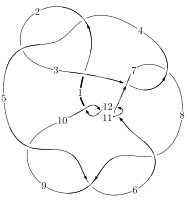
\includegraphics[width=112pt]{../../../GIT/diagram.site/Diagrams/png/2268_12n_0179.png}\\
\ \ \ A knot diagram\footnotemark}&
\allowdisplaybreaks
\textbf{Linearized knot diagam} \\
\cline{2-2}
 &
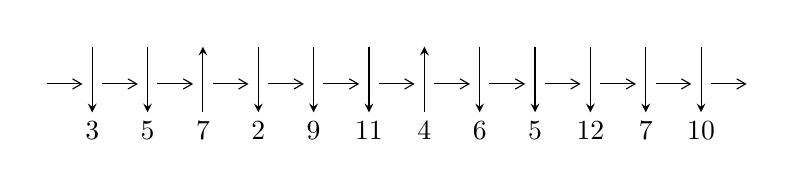
\begin{tikzpicture}[x=20pt, y=17pt]
	% nodes
	\node (C0) at (0, 0) {};
	\node (C1) at (1, 0) {};
	\node (C1U) at (1, +1) {};
	\node (C1D) at (1, -1) {3};

	\node (C2) at (2, 0) {};
	\node (C2U) at (2, +1) {};
	\node (C2D) at (2, -1) {5};

	\node (C3) at (3, 0) {};
	\node (C3U) at (3, +1) {};
	\node (C3D) at (3, -1) {7};

	\node (C4) at (4, 0) {};
	\node (C4U) at (4, +1) {};
	\node (C4D) at (4, -1) {2};

	\node (C5) at (5, 0) {};
	\node (C5U) at (5, +1) {};
	\node (C5D) at (5, -1) {9};

	\node (C6) at (6, 0) {};
	\node (C6U) at (6, +1) {};
	\node (C6D) at (6, -1) {11};

	\node (C7) at (7, 0) {};
	\node (C7U) at (7, +1) {};
	\node (C7D) at (7, -1) {4};

	\node (C8) at (8, 0) {};
	\node (C8U) at (8, +1) {};
	\node (C8D) at (8, -1) {6};

	\node (C9) at (9, 0) {};
	\node (C9U) at (9, +1) {};
	\node (C9D) at (9, -1) {5};

	\node (C10) at (10, 0) {};
	\node (C10U) at (10, +1) {};
	\node (C10D) at (10, -1) {12};

	\node (C11) at (11, 0) {};
	\node (C11U) at (11, +1) {};
	\node (C11D) at (11, -1) {7};

	\node (C12) at (12, 0) {};
	\node (C12U) at (12, +1) {};
	\node (C12D) at (12, -1) {10};
	\node (C13) at (13, 0) {};

	% arrows
	\draw[->,>={angle 60}]
	(C0) edge (C1) (C1) edge (C2) (C2) edge (C3) (C3) edge (C4) (C4) edge (C5) (C5) edge (C6) (C6) edge (C7) (C7) edge (C8) (C8) edge (C9) (C9) edge (C10) (C10) edge (C11) (C11) edge (C12) (C12) edge (C13) ;	\draw[->,>=stealth]
	(C1U) edge (C1D) (C2U) edge (C2D) (C3D) edge (C3U) (C4U) edge (C4D) (C5U) edge (C5D) (C6U) edge (C6D) (C7D) edge (C7U) (C8U) edge (C8D) (C9U) edge (C9D) (C10U) edge (C10D) (C11U) edge (C11D) (C12U) edge (C12D) ;
	\end{tikzpicture} \\
\hhline{~~} \\& 
\textbf{Solving Sequence} \\ \cline{2-2} 
 &
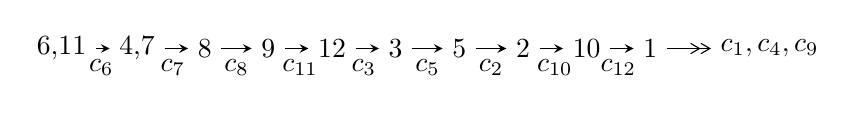
\begin{tikzpicture}[x=23pt, y=7pt]
	% node
	\node (A0) at (-1/8, 0) {6,11};
	\node (A1) at (17/16, 0) {4,7};
	\node (A2) at (17/8, 0) {8};
	\node (A3) at (25/8, 0) {9};
	\node (A4) at (33/8, 0) {12};
	\node (A5) at (41/8, 0) {3};
	\node (A6) at (49/8, 0) {5};
	\node (A7) at (57/8, 0) {2};
	\node (A8) at (65/8, 0) {10};
	\node (A9) at (73/8, 0) {1};
	\node (C1) at (1/2, -1) {$c_{6}$};
	\node (C2) at (13/8, -1) {$c_{7}$};
	\node (C3) at (21/8, -1) {$c_{8}$};
	\node (C4) at (29/8, -1) {$c_{11}$};
	\node (C5) at (37/8, -1) {$c_{3}$};
	\node (C6) at (45/8, -1) {$c_{5}$};
	\node (C7) at (53/8, -1) {$c_{2}$};
	\node (C8) at (61/8, -1) {$c_{10}$};
	\node (C9) at (69/8, -1) {$c_{12}$};
	\node (A10) at (11, 0) {$c_{1},c_{4},c_{9}$};

	% edge
	\draw[->,>=stealth]	
	(A0) edge (A1) (A1) edge (A2) (A2) edge (A3) (A3) edge (A4) (A4) edge (A5) (A5) edge (A6) (A6) edge (A7) (A7) edge (A8) (A8) edge (A9) ;
	\draw[->>,>={angle 60}]	
	(A9) edge (A10);
\end{tikzpicture} \\ 

\end{tabular} \\

\footnotetext{
The image of knot diagram is generated by the software ``\textbf{Draw programme}" developed by Andrew Bartholomew(\url{http://www.layer8.co.uk/maths/draw/index.htm\#Running-draw}), where we modified some parts for our purpose(\url{https://github.com/CATsTAILs/LinksPainter}).
}\phantom \\ \newline 
\centering \textbf{Ideals for irreducible components\footnotemark of $X_{\text{par}}$} 
 
\begin{align*}
I^u_{1}&=\langle 
1.37190\times10^{18} u^{22}-7.99565\times10^{18} u^{21}+\cdots+2.02541\times10^{20} b-2.79533\times10^{20},\\
\phantom{I^u_{1}}&\phantom{= \langle  }-4.59710\times10^{19} u^{22}-4.62744\times10^{20} u^{21}+\cdots+3.44319\times10^{21} a-1.63572\times10^{22},\\
\phantom{I^u_{1}}&\phantom{= \langle  }u^{23}+2 u^{22}+\cdots+52 u+17\rangle \\
I^u_{2}&=\langle 
-5 u^3 a^2-3 a^2 u^2+6 u^3 a+18 a^2 u+11 u^2 a-4 u^3-4 a^2-29 a u-32 u^2+37 b-10 a+7 u+19,\\
\phantom{I^u_{2}}&\phantom{= \langle  }2 u^3 a^2+2 a^2 u^2- u^3 a+a^3+a^2 u+2 u^3-2 a^2- a u+3 u^2+4 u+2,\;u^4- u^2+1\rangle \\
I^u_{3}&=\langle 
u^3- u^2+b+1,\;u^4- u^2+a+2 u+1,\;u^5- u^4+u^2+u-1\rangle \\
\\
\end{align*}
\raggedright * 3 irreducible components of $\dim_{\mathbb{C}}=0$, with total 40 representations.\\
\footnotetext{All coefficients of polynomials are rational numbers. But the coefficients are sometimes approximated in decimal forms when there is not enough margin.}
\newpage
\renewcommand{\arraystretch}{1}
\centering \section*{I. $I^u_{1}= \langle 1.37\times10^{18} u^{22}-8.00\times10^{18} u^{21}+\cdots+2.03\times10^{20} b-2.80\times10^{20},\;-4.60\times10^{19} u^{22}-4.63\times10^{20} u^{21}+\cdots+3.44\times10^{21} a-1.64\times10^{22},\;u^{23}+2 u^{22}+\cdots+52 u+17 \rangle$}
\flushleft \textbf{(i) Arc colorings}\\
\begin{tabular}{m{7pt} m{180pt} m{7pt} m{180pt} }
\flushright $a_{6}=$&$\begin{pmatrix}1\\0\end{pmatrix}$ \\
\flushright $a_{11}=$&$\begin{pmatrix}0\\u\end{pmatrix}$ \\
\flushright $a_{4}=$&$\begin{pmatrix}0.0133513 u^{22}+0.134394 u^{21}+\cdots-1.65131 u+4.75059\\-0.00677343 u^{22}+0.0394767 u^{21}+\cdots-0.213063 u+1.38013\end{pmatrix}$ \\
\flushright $a_{7}=$&$\begin{pmatrix}1\\u^2\end{pmatrix}$ \\
\flushright $a_{8}=$&$\begin{pmatrix}-0.415260 u^{22}-0.446011 u^{21}+\cdots-13.3132 u-7.56780\\-0.164479 u^{22}-0.153676 u^{21}+\cdots-4.53967 u-2.55254\end{pmatrix}$ \\
\flushright $a_{9}=$&$\begin{pmatrix}-0.250781 u^{22}-0.292335 u^{21}+\cdots-8.77357 u-5.01526\\-0.164479 u^{22}-0.153676 u^{21}+\cdots-4.53967 u-2.55254\end{pmatrix}$ \\
\flushright $a_{12}=$&$\begin{pmatrix}- u\\- u^3+u\end{pmatrix}$ \\
\flushright $a_{3}=$&$\begin{pmatrix}-0.158366 u^{22}-0.0384582 u^{21}+\cdots-7.26516 u+1.53971\\-0.184168 u^{22}-0.141177 u^{21}+\cdots-6.16412 u-1.51976\end{pmatrix}$ \\
\flushright $a_{5}=$&$\begin{pmatrix}0.191837 u^{22}+0.133885 u^{21}+\cdots+5.40801 u+3.14823\\0.0435720 u^{22}+0.0231293 u^{21}+\cdots+1.06482 u+0.103017\end{pmatrix}$ \\
\flushright $a_{2}=$&$\begin{pmatrix}-0.0136483 u^{22}+0.162115 u^{21}+\cdots-1.72543 u+5.96673\\-0.0408799 u^{22}+0.00329935 u^{21}+\cdots-0.954342 u+0.923420\end{pmatrix}$ \\
\flushright $a_{10}=$&$\begin{pmatrix}u^3\\u^5- u^3+u\end{pmatrix}$ \\
\flushright $a_{1}=$&$\begin{pmatrix}- u^5- u\\- u^7+u^5-2 u^3+u\end{pmatrix}$\\&\end{tabular}
\flushleft \textbf{(ii) Obstruction class $= -1$}\\~\\
\flushleft \textbf{(iii) Cusp Shapes $= \frac{45183703312586503683}{101270439284454752258} u^{22}+\frac{93456001880784428205}{101270439284454752258} u^{21}+\cdots+\frac{880293744256233854306}{50635219642227376129} u+\frac{601972144725743861757}{50635219642227376129}$}\\~\\
\newpage\renewcommand{\arraystretch}{1}
\flushleft \textbf{(iv) u-Polynomials at the component}\newline \\
\begin{tabular}{m{50pt}|m{274pt}}
Crossings & \hspace{64pt}u-Polynomials at each crossing \\
\hline $$\begin{aligned}c_{1}\end{aligned}$$&$\begin{aligned}
&u^{23}+28 u^{22}+\cdots-74 u+1
\end{aligned}$\\
\hline $$\begin{aligned}c_{2},c_{4}\end{aligned}$$&$\begin{aligned}
&u^{23}-10 u^{22}+\cdots+22 u-1
\end{aligned}$\\
\hline $$\begin{aligned}c_{3},c_{7}\end{aligned}$$&$\begin{aligned}
&u^{23}- u^{22}+\cdots-64 u-32
\end{aligned}$\\
\hline $$\begin{aligned}c_{5},c_{8},c_{9}\end{aligned}$$&$\begin{aligned}
&u^{23}-2 u^{22}+\cdots-238 u-49
\end{aligned}$\\
\hline $$\begin{aligned}c_{6},c_{11}\end{aligned}$$&$\begin{aligned}
&u^{23}-2 u^{22}+\cdots+52 u-17
\end{aligned}$\\
\hline $$\begin{aligned}c_{10},c_{12}\end{aligned}$$&$\begin{aligned}
&u^{23}+18 u^{22}+\cdots+3418 u+289
\end{aligned}$\\
\hline
\end{tabular}\\~\\
\newpage\renewcommand{\arraystretch}{1}
\flushleft \textbf{(v) Riley Polynomials at the component}\newline \\
\begin{tabular}{m{50pt}|m{274pt}}
Crossings & \hspace{64pt}Riley Polynomials at each crossing \\
\hline $$\begin{aligned}c_{1}\end{aligned}$$&$\begin{aligned}
&y^{23}-104 y^{22}+\cdots-62214 y-1
\end{aligned}$\\
\hline $$\begin{aligned}c_{2},c_{4}\end{aligned}$$&$\begin{aligned}
&y^{23}-28 y^{22}+\cdots-74 y-1
\end{aligned}$\\
\hline $$\begin{aligned}c_{3},c_{7}\end{aligned}$$&$\begin{aligned}
&y^{23}+21 y^{22}+\cdots+37376 y-1024
\end{aligned}$\\
\hline $$\begin{aligned}c_{5},c_{8},c_{9}\end{aligned}$$&$\begin{aligned}
&y^{23}+30 y^{21}+\cdots+31556 y-2401
\end{aligned}$\\
\hline $$\begin{aligned}c_{6},c_{11}\end{aligned}$$&$\begin{aligned}
&y^{23}-18 y^{22}+\cdots+3418 y-289
\end{aligned}$\\
\hline $$\begin{aligned}c_{10},c_{12}\end{aligned}$$&$\begin{aligned}
&y^{23}-18 y^{22}+\cdots+2928914 y-83521
\end{aligned}$\\
\hline
\end{tabular}\\~\\
\newpage\flushleft \textbf{(vi) Complex Volumes and Cusp Shapes}
$$\begin{array}{c|c|c}  
\text{Solutions to }I^u_{1}& \I (\text{vol} + \sqrt{-1}CS) & \text{Cusp shape}\\
 \hline 
\begin{aligned}
u &= -1.030250 + 0.133808 I \\
a &= \phantom{-}0.762093 + 1.177250 I \\
b &= -0.359850 + 0.929573 I\end{aligned}
 & \phantom{-}3.40068 - 2.08292 I & -6.94504 + 2.82033 I \\ \hline\begin{aligned}
u &= -1.030250 - 0.133808 I \\
a &= \phantom{-}0.762093 - 1.177250 I \\
b &= -0.359850 - 0.929573 I\end{aligned}
 & \phantom{-}3.40068 + 2.08292 I & -6.94504 - 2.82033 I \\ \hline\begin{aligned}
u &= \phantom{-}0.901962 + 0.543040 I \\
a &= \phantom{-}4.80515 + 0.32829 I \\
b &= \phantom{-}2.51685 + 4.97104 I\end{aligned}
 & -0.09172 - 2.05272 I & \phantom{-}13.5502 - 11.7426 I \\ \hline\begin{aligned}
u &= \phantom{-}0.901962 - 0.543040 I \\
a &= \phantom{-}4.80515 - 0.32829 I \\
b &= \phantom{-}2.51685 - 4.97104 I\end{aligned}
 & -0.09172 + 2.05272 I & \phantom{-}13.5502 + 11.7426 I \\ \hline\begin{aligned}
u &= -0.774138 + 0.517283 I \\
a &= -0.187723 - 0.729816 I \\
b &= -0.888501 - 0.210493 I\end{aligned}
 & \phantom{-}1.78208 + 2.09879 I & \phantom{-}0.37186 - 4.32801 I \\ \hline\begin{aligned}
u &= -0.774138 - 0.517283 I \\
a &= -0.187723 + 0.729816 I \\
b &= -0.888501 + 0.210493 I\end{aligned}
 & \phantom{-}1.78208 - 2.09879 I & \phantom{-}0.37186 + 4.32801 I \\ \hline\begin{aligned}
u &= -0.987737 + 0.455591 I \\
a &= \phantom{-}0.000748 - 1.386780 I \\
b &= \phantom{-}0.203991 - 0.922058 I\end{aligned}
 & \phantom{-}3.17947 + 4.60678 I & -8.98911 - 4.52953 I \\ \hline\begin{aligned}
u &= -0.987737 - 0.455591 I \\
a &= \phantom{-}0.000748 + 1.386780 I \\
b &= \phantom{-}0.203991 + 0.922058 I\end{aligned}
 & \phantom{-}3.17947 - 4.60678 I & -8.98911 + 4.52953 I \\ \hline\begin{aligned}
u &= \phantom{-}0.751562\phantom{ +0.000000I} \\
a &= -0.430119\phantom{ +0.000000I} \\
b &= \phantom{-}0.215899\phantom{ +0.000000I}\end{aligned}
 & -1.11111\phantom{ +0.000000I} & -8.83030\phantom{ +0.000000I} \\ \hline\begin{aligned}
u &= \phantom{-}0.913312 + 0.995998 I \\
a &= -0.455968 - 0.165528 I \\
b &= \phantom{-}0.0273478 + 0.1092730 I\end{aligned}
 & \phantom{-}8.77314 - 3.60069 I & -8.75891 + 4.90863 I\\
 \hline 
 \end{array}$$\newpage$$\begin{array}{c|c|c}  
\text{Solutions to }I^u_{1}& \I (\text{vol} + \sqrt{-1}CS) & \text{Cusp shape}\\
 \hline 
\begin{aligned}
u &= \phantom{-}0.913312 - 0.995998 I \\
a &= -0.455968 + 0.165528 I \\
b &= \phantom{-}0.0273478 - 0.1092730 I\end{aligned}
 & \phantom{-}8.77314 + 3.60069 I & -8.75891 - 4.90863 I \\ \hline\begin{aligned}
u &= -0.29230 + 1.39423 I \\
a &= \phantom{-}0.306239 - 0.296422 I \\
b &= \phantom{-}0.27422 - 1.73853 I\end{aligned}
 & -9.67128 - 5.78622 I & -6.43045 + 2.03811 I \\ \hline\begin{aligned}
u &= -0.29230 - 1.39423 I \\
a &= \phantom{-}0.306239 + 0.296422 I \\
b &= \phantom{-}0.27422 + 1.73853 I\end{aligned}
 & -9.67128 + 5.78622 I & -6.43045 - 2.03811 I \\ \hline\begin{aligned}
u &= \phantom{-}0.312134 + 0.458419 I \\
a &= -0.517712 - 0.280214 I \\
b &= \phantom{-}0.099441 + 0.699809 I\end{aligned}
 & -0.646445 - 1.161780 I & -6.90693 + 5.27856 I \\ \hline\begin{aligned}
u &= \phantom{-}0.312134 - 0.458419 I \\
a &= -0.517712 + 0.280214 I \\
b &= \phantom{-}0.099441 - 0.699809 I\end{aligned}
 & -0.646445 + 1.161780 I & -6.90693 - 5.27856 I \\ \hline\begin{aligned}
u &= -1.34978 + 0.77312 I \\
a &= -0.81654 + 1.45288 I \\
b &= \phantom{-}0.50785 + 1.97781 I\end{aligned}
 & -12.9726 + 13.2355 I & -7.13536 - 5.53565 I \\ \hline\begin{aligned}
u &= -1.34978 - 0.77312 I \\
a &= -0.81654 - 1.45288 I \\
b &= \phantom{-}0.50785 - 1.97781 I\end{aligned}
 & -12.9726 - 13.2355 I & -7.13536 + 5.53565 I \\ \hline\begin{aligned}
u &= -0.377835\phantom{ +0.000000I} \\
a &= \phantom{-}3.52955\phantom{ +0.000000I} \\
b &= \phantom{-}0.965970\phantom{ +0.000000I}\end{aligned}
 & -2.11000\phantom{ +0.000000I} & \phantom{-}0.409770\phantom{ +0.000000I} \\ \hline\begin{aligned}
u &= -1.59039 + 0.40688 I \\
a &= \phantom{-}0.35471 - 1.57413 I \\
b &= -0.18308 - 1.79179 I\end{aligned}
 & -6.97074 + 4.93755 I & -7.69369 - 2.56266 I \\ \hline\begin{aligned}
u &= -1.59039 - 0.40688 I \\
a &= \phantom{-}0.35471 + 1.57413 I \\
b &= -0.18308 + 1.79179 I\end{aligned}
 & -6.97074 - 4.93755 I & -7.69369 + 2.56266 I\\
 \hline 
 \end{array}$$\newpage$$\begin{array}{c|c|c}  
\text{Solutions to }I^u_{1}& \I (\text{vol} + \sqrt{-1}CS) & \text{Cusp shape}\\
 \hline 
\begin{aligned}
u &= \phantom{-}1.78874\phantom{ +0.000000I} \\
a &= \phantom{-}0.851439\phantom{ +0.000000I} \\
b &= -0.299287\phantom{ +0.000000I}\end{aligned}
 & -10.2305\phantom{ +0.000000I} & -8.74930\phantom{ +0.000000I} \\ \hline\begin{aligned}
u &= \phantom{-}1.81595 + 0.61002 I \\
a &= \phantom{-}0.714754 + 1.134980 I \\
b &= -0.13957 + 1.61563 I\end{aligned}
 & -16.2453 - 1.7569 I & -8.47765 + 0.68383 I \\ \hline\begin{aligned}
u &= \phantom{-}1.81595 - 0.61002 I \\
a &= \phantom{-}0.714754 - 1.134980 I \\
b &= -0.13957 - 1.61563 I\end{aligned}
 & -16.2453 + 1.7569 I & -8.47765 - 0.68383 I\\
 \hline 
 \end{array}$$\newpage\newpage\renewcommand{\arraystretch}{1}
\centering \section*{II. $I^u_{2}= \langle -5 u^3 a^2+6 u^3 a+\cdots-10 a+19,\;2 u^3 a^2- u^3 a+\cdots-2 a^2+2,\;u^4- u^2+1 \rangle$}
\flushleft \textbf{(i) Arc colorings}\\
\begin{tabular}{m{7pt} m{180pt} m{7pt} m{180pt} }
\flushright $a_{6}=$&$\begin{pmatrix}1\\0\end{pmatrix}$ \\
\flushright $a_{11}=$&$\begin{pmatrix}0\\u\end{pmatrix}$ \\
\flushright $a_{4}=$&$\begin{pmatrix}a\\0.135135 a^{2} u^{3}-0.162162 a u^{3}+\cdots+0.270270 a-0.513514\end{pmatrix}$ \\
\flushright $a_{7}=$&$\begin{pmatrix}1\\u^2\end{pmatrix}$ \\
\flushright $a_{8}=$&$\begin{pmatrix}-0.351351 a^{2} u^{3}-0.378378 a u^{3}+\cdots+0.297297 a+1.13514\\- u^3\end{pmatrix}$ \\
\flushright $a_{9}=$&$\begin{pmatrix}-0.351351 a^{2} u^{3}-0.378378 a u^{3}+\cdots+0.297297 a+1.13514\\- u^3\end{pmatrix}$ \\
\flushright $a_{12}=$&$\begin{pmatrix}- u\\- u^3+u\end{pmatrix}$ \\
\flushright $a_{3}=$&$\begin{pmatrix}-0.135135 a^{2} u^{3}+0.162162 a u^{3}+\cdots+0.729730 a+0.513514\\0.486486 a^{2} u^{3}-0.783784 a u^{3}+\cdots-1.02703 a+0.351351\end{pmatrix}$ \\
\flushright $a_{5}=$&$\begin{pmatrix}0.108108 a^{2} u^{3}+0.270270 a u^{3}+\cdots+0.216216 a+1.18919\\1\end{pmatrix}$ \\
\flushright $a_{2}=$&$\begin{pmatrix}0.0270270 a^{2} u^{3}+0.567568 a u^{3}+\cdots+0.0540541 a+1.29730\\-0.189189 a^{2} u^{3}+0.0270270 a u^{3}+\cdots-0.378378 a+0.918919\end{pmatrix}$ \\
\flushright $a_{10}=$&$\begin{pmatrix}u^3\\0\end{pmatrix}$ \\
\flushright $a_{1}=$&$\begin{pmatrix}- u^3\\- u^3+u\end{pmatrix}$\\&\end{tabular}
\flushleft \textbf{(ii) Obstruction class $= 1$}\\~\\
\flushleft \textbf{(iii) Cusp Shapes $= -\frac{100}{37} u^3 a^2+\frac{88}{37} a^2 u^2+\frac{120}{37} u^3 a+\frac{64}{37} a^2 u-\frac{76}{37} u^2 a-\frac{80}{37} u^3-\frac{80}{37} a^2-\frac{136}{37} a u+\frac{100}{37} u^2+\frac{96}{37} a+\frac{140}{37} u-\frac{212}{37}$}\\~\\
\newpage\renewcommand{\arraystretch}{1}
\flushleft \textbf{(iv) u-Polynomials at the component}\newline \\
\begin{tabular}{m{50pt}|m{274pt}}
Crossings & \hspace{64pt}u-Polynomials at each crossing \\
\hline $$\begin{aligned}c_{1}\end{aligned}$$&$\begin{aligned}
&(u^3- u^2+2 u-1)^4
\end{aligned}$\\
\hline $$\begin{aligned}c_{2}\end{aligned}$$&$\begin{aligned}
&(u^3+u^2-1)^4
\end{aligned}$\\
\hline $$\begin{aligned}c_{3},c_{7}\end{aligned}$$&$\begin{aligned}
&(u^6-3 u^4+2 u^2+1)^2
\end{aligned}$\\
\hline $$\begin{aligned}c_{4}\end{aligned}$$&$\begin{aligned}
&(u^3- u^2+1)^4
\end{aligned}$\\
\hline $$\begin{aligned}c_{5},c_{8},c_{9}\end{aligned}$$&$\begin{aligned}
&(u^2+1)^6
\end{aligned}$\\
\hline $$\begin{aligned}c_{6},c_{11}\end{aligned}$$&$\begin{aligned}
&(u^4- u^2+1)^3
\end{aligned}$\\
\hline $$\begin{aligned}c_{10}\end{aligned}$$&$\begin{aligned}
&(u^2- u+1)^6
\end{aligned}$\\
\hline $$\begin{aligned}c_{12}\end{aligned}$$&$\begin{aligned}
&(u^2+u+1)^6
\end{aligned}$\\
\hline
\end{tabular}\\~\\
\newpage\renewcommand{\arraystretch}{1}
\flushleft \textbf{(v) Riley Polynomials at the component}\newline \\
\begin{tabular}{m{50pt}|m{274pt}}
Crossings & \hspace{64pt}Riley Polynomials at each crossing \\
\hline $$\begin{aligned}c_{1}\end{aligned}$$&$\begin{aligned}
&(y^3+3 y^2+2 y-1)^4
\end{aligned}$\\
\hline $$\begin{aligned}c_{2},c_{4}\end{aligned}$$&$\begin{aligned}
&(y^3- y^2+2 y-1)^4
\end{aligned}$\\
\hline $$\begin{aligned}c_{3},c_{7}\end{aligned}$$&$\begin{aligned}
&(y^3-3 y^2+2 y+1)^4
\end{aligned}$\\
\hline $$\begin{aligned}c_{5},c_{8},c_{9}\end{aligned}$$&$\begin{aligned}
&(y+1)^{12}
\end{aligned}$\\
\hline $$\begin{aligned}c_{6},c_{11}\end{aligned}$$&$\begin{aligned}
&(y^2- y+1)^6
\end{aligned}$\\
\hline $$\begin{aligned}c_{10},c_{12}\end{aligned}$$&$\begin{aligned}
&(y^2+y+1)^6
\end{aligned}$\\
\hline
\end{tabular}\\~\\
\newpage\flushleft \textbf{(vi) Complex Volumes and Cusp Shapes}
$$\begin{array}{c|c|c}  
\text{Solutions to }I^u_{2}& \I (\text{vol} + \sqrt{-1}CS) & \text{Cusp shape}\\
 \hline 
\begin{aligned}
u &= \phantom{-}0.866025 + 0.500000 I \\
a &= \phantom{-}0.611376 + 1.168210 I \\
b &= \phantom{-}0.60113 + 1.32865 I\end{aligned}
 & \phantom{-}4.66906 + 0.79824 I & -2.49024 + 0.48465 I \\ \hline\begin{aligned}
u &= \phantom{-}0.866025 + 0.500000 I \\
a &= -0.86134 - 1.84069 I \\
b &= -0.14373 - 1.45121 I\end{aligned}
 & \phantom{-}4.66906 - 4.85801 I & -2.49024 + 6.44355 I \\ \hline\begin{aligned}
u &= \phantom{-}0.866025 + 0.500000 I \\
a &= \phantom{-}0.38394 - 3.55957 I \\
b &= \phantom{-}3.27465 - 0.87744 I\end{aligned}
 & \phantom{-}0.53148 - 2.02988 I & -9.01951 + 3.46410 I \\ \hline\begin{aligned}
u &= \phantom{-}0.866025 - 0.500000 I \\
a &= \phantom{-}0.611376 - 1.168210 I \\
b &= \phantom{-}0.60113 - 1.32865 I\end{aligned}
 & \phantom{-}4.66906 - 0.79824 I & -2.49024 - 0.48465 I \\ \hline\begin{aligned}
u &= \phantom{-}0.866025 - 0.500000 I \\
a &= -0.86134 + 1.84069 I \\
b &= -0.14373 + 1.45121 I\end{aligned}
 & \phantom{-}4.66906 + 4.85801 I & -2.49024 - 6.44355 I \\ \hline\begin{aligned}
u &= \phantom{-}0.866025 - 0.500000 I \\
a &= \phantom{-}0.38394 + 3.55957 I \\
b &= \phantom{-}3.27465 + 0.87744 I\end{aligned}
 & \phantom{-}0.53148 + 2.02988 I & -9.01951 - 3.46410 I \\ \hline\begin{aligned}
u &= -0.866025 + 0.500000 I \\
a &= \phantom{-}0.801323 + 0.635627 I \\
b &= -0.356011 - 0.161073 I\end{aligned}
 & \phantom{-}4.66906 - 0.79824 I & -2.49024 - 0.48465 I \\ \hline\begin{aligned}
u &= -0.866025 + 0.500000 I \\
a &= -0.306233 - 0.883547 I \\
b &= \phantom{-}0.388851 + 0.038512 I\end{aligned}
 & \phantom{-}4.66906 + 4.85801 I & -2.49024 - 6.44355 I \\ \hline\begin{aligned}
u &= -0.866025 + 0.500000 I \\
a &= \phantom{-}1.37094 - 0.52003 I \\
b &= \phantom{-}0.235109 - 0.877439 I\end{aligned}
 & \phantom{-}0.53148 + 2.02988 I & -9.01951 - 3.46410 I \\ \hline\begin{aligned}
u &= -0.866025 - 0.500000 I \\
a &= \phantom{-}0.801323 - 0.635627 I \\
b &= -0.356011 + 0.161073 I\end{aligned}
 & \phantom{-}4.66906 + 0.79824 I & -2.49024 + 0.48465 I\\
 \hline 
 \end{array}$$\newpage$$\begin{array}{c|c|c}  
\text{Solutions to }I^u_{2}& \I (\text{vol} + \sqrt{-1}CS) & \text{Cusp shape}\\
 \hline 
\begin{aligned}
u &= -0.866025 - 0.500000 I \\
a &= -0.306233 + 0.883547 I \\
b &= \phantom{-}0.388851 - 0.038512 I\end{aligned}
 & \phantom{-}4.66906 - 4.85801 I & -2.49024 + 6.44355 I \\ \hline\begin{aligned}
u &= -0.866025 - 0.500000 I \\
a &= \phantom{-}1.37094 + 0.52003 I \\
b &= \phantom{-}0.235109 + 0.877439 I\end{aligned}
 & \phantom{-}0.53148 - 2.02988 I & -9.01951 + 3.46410 I\\
 \hline 
 \end{array}$$\newpage\newpage\renewcommand{\arraystretch}{1}
\centering \section*{III. $I^u_{3}= \langle u^3- u^2+b+1,\;u^4- u^2+a+2 u+1,\;u^5- u^4+u^2+u-1 \rangle$}
\flushleft \textbf{(i) Arc colorings}\\
\begin{tabular}{m{7pt} m{180pt} m{7pt} m{180pt} }
\flushright $a_{6}=$&$\begin{pmatrix}1\\0\end{pmatrix}$ \\
\flushright $a_{11}=$&$\begin{pmatrix}0\\u\end{pmatrix}$ \\
\flushright $a_{4}=$&$\begin{pmatrix}- u^4+u^2-2 u-1\\- u^3+u^2-1\end{pmatrix}$ \\
\flushright $a_{7}=$&$\begin{pmatrix}1\\u^2\end{pmatrix}$ \\
\flushright $a_{8}=$&$\begin{pmatrix}1\\u^2\end{pmatrix}$ \\
\flushright $a_{9}=$&$\begin{pmatrix}- u^2+1\\u^2\end{pmatrix}$ \\
\flushright $a_{12}=$&$\begin{pmatrix}- u\\- u^3+u\end{pmatrix}$ \\
\flushright $a_{3}=$&$\begin{pmatrix}- u^4+u^2-2 u-1\\- u^3+u^2-1\end{pmatrix}$ \\
\flushright $a_{5}=$&$\begin{pmatrix}u^4- u^2+1\\- u^4\end{pmatrix}$ \\
\flushright $a_{2}=$&$\begin{pmatrix}-2 u^4+2 u^2-2 u-2\\u^4- u^3+u^2-1\end{pmatrix}$ \\
\flushright $a_{10}=$&$\begin{pmatrix}u^3\\u^4- u^3- u^2+1\end{pmatrix}$ \\
\flushright $a_{1}=$&$\begin{pmatrix}- u^4+u^2-1\\u^4\end{pmatrix}$\\&\end{tabular}
\flushleft \textbf{(ii) Obstruction class $= 1$}\\~\\
\flushleft \textbf{(iii) Cusp Shapes $= -9 u^4+u^3+2 u^2-4 u-17$}\\~\\
\newpage\renewcommand{\arraystretch}{1}
\flushleft \textbf{(iv) u-Polynomials at the component}\newline \\
\begin{tabular}{m{50pt}|m{274pt}}
Crossings & \hspace{64pt}u-Polynomials at each crossing \\
\hline $$\begin{aligned}c_{1},c_{2}\end{aligned}$$&$\begin{aligned}
&(u-1)^5
\end{aligned}$\\
\hline $$\begin{aligned}c_{3},c_{7}\end{aligned}$$&$\begin{aligned}
&u^5
\end{aligned}$\\
\hline $$\begin{aligned}c_{4}\end{aligned}$$&$\begin{aligned}
&(u+1)^5
\end{aligned}$\\
\hline $$\begin{aligned}c_{5},c_{10}\end{aligned}$$&$\begin{aligned}
&u^5- u^4+4 u^3-3 u^2+3 u-1
\end{aligned}$\\
\hline $$\begin{aligned}c_{6}\end{aligned}$$&$\begin{aligned}
&u^5- u^4+u^2+u-1
\end{aligned}$\\
\hline $$\begin{aligned}c_{8},c_{9},c_{12}\end{aligned}$$&$\begin{aligned}
&u^5+u^4+4 u^3+3 u^2+3 u+1
\end{aligned}$\\
\hline $$\begin{aligned}c_{11}\end{aligned}$$&$\begin{aligned}
&u^5+u^4- u^2+u+1
\end{aligned}$\\
\hline
\end{tabular}\\~\\
\newpage\renewcommand{\arraystretch}{1}
\flushleft \textbf{(v) Riley Polynomials at the component}\newline \\
\begin{tabular}{m{50pt}|m{274pt}}
Crossings & \hspace{64pt}Riley Polynomials at each crossing \\
\hline $$\begin{aligned}c_{1},c_{2},c_{4}\end{aligned}$$&$\begin{aligned}
&(y-1)^5
\end{aligned}$\\
\hline $$\begin{aligned}c_{3},c_{7}\end{aligned}$$&$\begin{aligned}
&y^5
\end{aligned}$\\
\hline $$\begin{aligned}c_{5},c_{8},c_{9}\\c_{10},c_{12}\end{aligned}$$&$\begin{aligned}
&y^5+7 y^4+16 y^3+13 y^2+3 y-1
\end{aligned}$\\
\hline $$\begin{aligned}c_{6},c_{11}\end{aligned}$$&$\begin{aligned}
&y^5- y^4+4 y^3-3 y^2+3 y-1
\end{aligned}$\\
\hline
\end{tabular}\\~\\
\newpage\flushleft \textbf{(vi) Complex Volumes and Cusp Shapes}
$$\begin{array}{c|c|c}  
\text{Solutions to }I^u_{3}& \I (\text{vol} + \sqrt{-1}CS) & \text{Cusp shape}\\
 \hline 
\begin{aligned}
u &= -0.758138 + 0.584034 I \\
a &= \phantom{-}1.47956 - 1.63976 I \\
b &= -1.10636 - 1.69341 I\end{aligned}
 & \phantom{-}0.17487 + 2.21397 I & -6.59361 + 0.42541 I \\ \hline\begin{aligned}
u &= -0.758138 - 0.584034 I \\
a &= \phantom{-}1.47956 + 1.63976 I \\
b &= -1.10636 + 1.69341 I\end{aligned}
 & \phantom{-}0.17487 - 2.21397 I & -6.59361 - 0.42541 I \\ \hline\begin{aligned}
u &= \phantom{-}0.935538 + 0.903908 I \\
a &= \phantom{-}0.044146 - 0.313338 I \\
b &= \phantom{-}0.532511 + 0.056433 I\end{aligned}
 & \phantom{-}9.31336 - 3.33174 I & \phantom{-}3.61324 - 0.36944 I \\ \hline\begin{aligned}
u &= \phantom{-}0.935538 - 0.903908 I \\
a &= \phantom{-}0.044146 + 0.313338 I \\
b &= \phantom{-}0.532511 - 0.056433 I\end{aligned}
 & \phantom{-}9.31336 + 3.33174 I & \phantom{-}3.61324 + 0.36944 I \\ \hline\begin{aligned}
u &= \phantom{-}0.645200\phantom{ +0.000000I} \\
a &= -2.04741\phantom{ +0.000000I} \\
b &= -0.852303\phantom{ +0.000000I}\end{aligned}
 & -2.52712\phantom{ +0.000000I} & -20.0390\phantom{ +0.000000I}\\
 \hline 
 \end{array}$$\newpage
\newpage\renewcommand{\arraystretch}{1}
\centering \section*{ IV. u-Polynomials}
\begin{tabular}{m{50pt}|m{274pt}}
Crossings & \hspace{64pt}u-Polynomials at each crossing \\
\hline $$\begin{aligned}c_{1}\end{aligned}$$&$\begin{aligned}
&((u-1)^5)(u^3- u^2+2 u-1)^4(u^{23}+28 u^{22}+\cdots-74 u+1)
\end{aligned}$\\
\hline $$\begin{aligned}c_{2}\end{aligned}$$&$\begin{aligned}
&((u-1)^5)(u^3+u^2-1)^4(u^{23}-10 u^{22}+\cdots+22 u-1)
\end{aligned}$\\
\hline $$\begin{aligned}c_{3},c_{7}\end{aligned}$$&$\begin{aligned}
&u^5(u^6-3 u^4+2 u^2+1)^2(u^{23}- u^{22}+\cdots-64 u-32)
\end{aligned}$\\
\hline $$\begin{aligned}c_{4}\end{aligned}$$&$\begin{aligned}
&((u+1)^5)(u^3- u^2+1)^4(u^{23}-10 u^{22}+\cdots+22 u-1)
\end{aligned}$\\
\hline $$\begin{aligned}c_{5}\end{aligned}$$&$\begin{aligned}
&((u^2+1)^6)(u^5- u^4+\cdots+3 u-1)(u^{23}-2 u^{22}+\cdots-238 u-49)
\end{aligned}$\\
\hline $$\begin{aligned}c_{6}\end{aligned}$$&$\begin{aligned}
&((u^4- u^2+1)^3)(u^5- u^4+u^2+u-1)(u^{23}-2 u^{22}+\cdots+52 u-17)
\end{aligned}$\\
\hline $$\begin{aligned}c_{8},c_{9}\end{aligned}$$&$\begin{aligned}
&((u^2+1)^6)(u^5+u^4+\cdots+3 u+1)(u^{23}-2 u^{22}+\cdots-238 u-49)
\end{aligned}$\\
\hline $$\begin{aligned}c_{10}\end{aligned}$$&$\begin{aligned}
&(u^2- u+1)^6(u^5- u^4+4 u^3-3 u^2+3 u-1)\\
&\cdot(u^{23}+18 u^{22}+\cdots+3418 u+289)
\end{aligned}$\\
\hline $$\begin{aligned}c_{11}\end{aligned}$$&$\begin{aligned}
&((u^4- u^2+1)^3)(u^5+u^4- u^2+u+1)(u^{23}-2 u^{22}+\cdots+52 u-17)
\end{aligned}$\\
\hline $$\begin{aligned}c_{12}\end{aligned}$$&$\begin{aligned}
&(u^2+u+1)^6(u^5+u^4+4 u^3+3 u^2+3 u+1)\\
&\cdot(u^{23}+18 u^{22}+\cdots+3418 u+289)
\end{aligned}$\\
\hline
\end{tabular}\newpage\renewcommand{\arraystretch}{1}
\centering \section*{ V. Riley Polynomials}
\begin{tabular}{m{50pt}|m{274pt}}
Crossings & \hspace{64pt}Riley Polynomials at each crossing \\
\hline $$\begin{aligned}c_{1}\end{aligned}$$&$\begin{aligned}
&((y-1)^5)(y^3+3 y^2+2 y-1)^4(y^{23}-104 y^{22}+\cdots-62214 y-1)
\end{aligned}$\\
\hline $$\begin{aligned}c_{2},c_{4}\end{aligned}$$&$\begin{aligned}
&((y-1)^5)(y^3- y^2+2 y-1)^4(y^{23}-28 y^{22}+\cdots-74 y-1)
\end{aligned}$\\
\hline $$\begin{aligned}c_{3},c_{7}\end{aligned}$$&$\begin{aligned}
&y^5(y^3-3 y^2+2 y+1)^4(y^{23}+21 y^{22}+\cdots+37376 y-1024)
\end{aligned}$\\
\hline $$\begin{aligned}c_{5},c_{8},c_{9}\end{aligned}$$&$\begin{aligned}
&(y+1)^{12}(y^5+7 y^4+16 y^3+13 y^2+3 y-1)\\
&\cdot(y^{23}+30 y^{21}+\cdots+31556 y-2401)
\end{aligned}$\\
\hline $$\begin{aligned}c_{6},c_{11}\end{aligned}$$&$\begin{aligned}
&(y^2- y+1)^6(y^5- y^4+4 y^3-3 y^2+3 y-1)\\
&\cdot(y^{23}-18 y^{22}+\cdots+3418 y-289)
\end{aligned}$\\
\hline $$\begin{aligned}c_{10},c_{12}\end{aligned}$$&$\begin{aligned}
&(y^2+y+1)^6(y^5+7 y^4+16 y^3+13 y^2+3 y-1)\\
&\cdot(y^{23}-18 y^{22}+\cdots+2928914 y-83521)
\end{aligned}$\\
\hline
\end{tabular}
\vskip 2pc
\end{document}